\documentclass[10pt,twocolumn]{article}

\usepackage[utf8]{inputenc}
\usepackage[T1]{fontenc}
\usepackage{times}
\usepackage{latexsym}
\usepackage{microtype}
\usepackage{amsmath}
\usepackage{amssymb}
\usepackage{booktabs}
\usepackage{geometry}
\usepackage{hyperref}
\usepackage{tcolorbox}
\usepackage{tikz}
\usepackage{pgfplots}
\usepackage{titlesec}
\usepackage{filecontents}
\usepackage[numbers,sort&compress]{natbib}
\usepackage{fancyhdr}

\geometry{letterpaper, left=2.0cm, right=2.0cm, top=2.5cm, bottom=2.5cm, columnsep=0.8cm, headheight=20pt}

\usetikzlibrary{positioning,calc}
\pgfplotsset{compat=1.18}

\definecolor{NavyBlue}{HTML}{1A365D}
\definecolor{Charcoal}{HTML}{2D3748}
\definecolor{MutedTeal}{HTML}{0D9488}
\definecolor{WarmGray}{HTML}{F7FAFC}
\definecolor{AlertRed}{HTML}{9B2C2C}
\definecolor{LightRed}{HTML}{FFF5F5}

\hypersetup{
    colorlinks=true,
    linkcolor=NavyBlue,
    filecolor=MutedTeal,      
    urlcolor=MutedTeal,
    citecolor=NavyBlue,
    pdfauthor={Sarah Chen, Elena Rostova, Marcus Vance, Arthur Pendelton},
    pdftitle={Cross-Lingual Knowledge Transfer in Ultra-Low Resource Scenarios via Synaptic Latent Mapping},
}

\titleformat{\section}{\large\bfseries\color{NavyBlue}}{\thesection}{0.6em}{}
\titleformat{\subsection}{\normalsize\bfseries\color{Charcoal}}{\thesubsection}{0.6em}{}
\titlespacing*{\section}{0pt}{12pt}{6pt}
\titlespacing*{\subsection}{0pt}{8pt}{4pt}

\pagestyle{fancy}
\fancyhf{}
\lhead{\small\color{Charcoal} Unofficial ACL 2026 Submission Template}
\rhead{\small\color{Charcoal} Fictional NLP Research Group}
\cfoot{\small\color{Charcoal}\thepage}
\renewcommand{\headrulewidth}{0.4pt}
\renewcommand{\headrule}{\hbox to\headwidth{\color{MutedTeal}\leaders\hrule height \headrulewidth\hfill}}

\renewenvironment{abstract}{
  \small\itshape
  \noindent\textbf{Abstract}---%
}{
  \par\vspace{1em}
}

% --- BIBLIOGRAPHY FILE CONTENTS ---
\begin{filecontents*}{\jobname.bib}
@article{chen2024latent,
  author    = {Chen, Sarah and Rostova, Elena},
  title     = {Nonlinear Manifold Alignment for Low-Resource Neural Machine Translation},
  journal   = {Journal of Vertex Artificial Intelligence Research},
  volume    = {14},
  number    = {3},
  pages     = {245--259},
  year      = {2024},
  publisher = {Vertex Press}
}

@inproceedings{vance2023synaptic,
  author    = {Vance, Marcus and Pendelton, Arthur},
  title     = {Synaptic Weights Projection for Multilingual Transfer Learning},
  booktitle = {Proceedings of the Apex Conference on Computational Linguistics},
  pages     = {112--121},
  year      = {2023}
}

@article{roberts2022meridian,
  author    = {Roberts, David and Sterling, Alistair},
  title     = {The Meridian Language Family: Dialectal Variations and Computational Corpora},
  journal   = {Nexa NLP Journal},
  volume    = {8},
  number    = {1},
  pages     = {45--68},
  year      = {2022}
}

@inproceedings{zhang2025crosslingual,
  author    = {Zhang, Min and Tanaka, Kenji},
  title     = {Unsupervised Cross-Lingual Word Embeddings for Ultra-Low Resource Dialects},
  booktitle = {Proceedings of the Synapse Systems Symposium},
  pages     = {402--411},
  year      = {2025}
}

@article{adams2021neural,
  author    = {Adams, Evelyn and Gomez, Carlos},
  title     = {Zero-Shot Transfer Learning in Multilingual Pre-trained Models},
  journal   = {Computational Linguistics and AI Quarterly},
  volume    = {37},
  number    = {4},
  pages     = {891--915},
  year      = {2021}
}

@inproceedings{pendelton2024nimbus,
  author    = {Pendelton, Arthur and Vance, Marcus},
  title     = {Nimbus-BERT: A Lightweight Multilingual Model for Low-Resource Languages},
  booktitle = {International Conference on Synapse Learning Representations},
  pages     = {1542--1551},
  year      = {2024}
}

@article{rostova2025topological,
  author    = {Rostova, Elena and Chen, Sarah},
  title     = {Topological Data Analysis for Deep Neural Space Mapping},
  journal   = {Meridian Computational Mathematics},
  volume    = {19},
  number    = {2},
  pages     = {130--148},
  year      = {2025}
}

@inproceedings{vance2025benchmarking,
  author    = {Vance, Marcus and Chen, Sarah and Rostova, Elena},
  title     = {Benchmarking Neural Machine Translation on the Meridian Dialect Suite},
  booktitle = {Proceedings of the Vertex NLP Workshop},
  pages     = {78--87},
  year      = {2025}
}

@article{miller2020transfer,
  author    = {Miller, James and Davis, Karen},
  title     = {An Analysis of Domain Adaptation Techniques in Deep Learning},
  journal   = {Apex Technical Journal},
  volume    = {42},
  number    = {5},
  pages     = {612--630},
  year      = {2020}
}

@inproceedings{nexa2024large,
  author    = {Nexa Research Group},
  title     = {Evaluating Large Language Models on Low-Resource Morphological Tasks},
  booktitle = {Proceedings of the Nimbus AI Summit},
  pages     = {99--108},
  year      = {2024}
}
\end{filecontents*}

\begin{document}

\twocolumn[
  \begin{center}
    \fcolorbox{AlertRed}{LightRed}{%
      \begin{minipage}{\dimexpr\linewidth-2\fboxsep-2\fboxrule\relax}
        \small\centering\color{AlertRed}
        \textbf{UNOFFICIAL TEMPLATE:} This document is not affiliated with, endorsed by, or sponsored by the Association for Computational Linguistics (ACL) or the ACL 2026 conference. Authors must consult the official ACL website and current year's style guide for camera-ready submission.
      \end{minipage}%
    }
    \vspace{1.5em}
    {\huge\bfseries\color{NavyBlue} Cross-Lingual Knowledge Transfer in Ultra-Low Resource Scenarios via Synaptic Latent Mapping \par}
    \vspace{1.5em}
    {\large
      \begin{tabular}{ccc}
        \textbf{Sarah Chen}$^{1}$ & \textbf{Elena Rostova}$^{2}$ & \textbf{Marcus Vance}$^{3}$ \\
        $^{1}$Synapse Technologies & $^{2}$Vertex Research & $^{3}$Apex Systems \\
        \texttt{s.chen@synapse.ai} & \texttt{rostova@vertex.org} & \texttt{vance@apex.tech}
      \end{tabular}
    \par}
    \vspace{1.0em}
    {\large
      \begin{tabular}{c}
        \textbf{Arthur Pendelton}$^{4}$ \\
        $^{4}$Nimbus AI Laboratory \\
        \texttt{pendelton@nimbus.com}
      \end{tabular}
    \par}
    \vspace{2.0em}
  \end{center}
]

\begin{abstract}
We present a novel approach to cross-lingual transfer learning under extreme resource constraints (fewer than 1,000 parallel sentences). Our method, \textbf{Synaptic Latent Mapping} (\textbf{SLM}), projects representations from a resource-rich source language into a target language's space by aligning low-dimensional topological manifolds. Unlike traditional mapping techniques that assume linear translation spaces, SLM leverages structural characteristics of deep neural networks to perform non-linear alignment. Experiments on five low-resource dialects from the Meridian language family show that SLM outperforms standard multilingual models by up to 4.2 BLEU points. Furthermore, we demonstrate that the aligned spaces can be transferred with minimal fine-tuning, paving the way for more equitable language technology.
\end{abstract}

\section{Introduction}
Natural Language Processing (NLP) has made substantial progress in recent years, driven by the emergence of large language models pre-trained on massive web-scale corpora. However, the benefits of these advances remain unevenly distributed. Out of the thousands of languages spoken worldwide, only a tiny fraction possess the resources required to train modern deep learning models from scratch. For languages with fewer than a few thousand pages of digitized text, standard pre-training techniques fail to build robust representations.

To bridge this digital divide, cross-lingual transfer learning has emerged as a major paradigm. By leveraging representations learned from high-resource source languages, researchers attempt to bootstrap models for low-resource target languages. However, existing methods such as linear mapping of word embeddings \citep{zhang2025crosslingual} or direct zero-shot transfer via massive multilingual models \citep{adams2021neural} often perform poorly on morphologically rich or highly divergent dialects.

In this work, we propose \textbf{Synaptic Latent Mapping} (\textbf{SLM}), a novel non-linear manifold alignment technique designed specifically for ultra-low resource scenarios. Our approach is based on the observation that deep neural network representations preserve fundamental semantic structures across languages, even if the absolute coordinate systems differ. By framing cross-lingual transfer as a topological alignment problem, we map the latent space of a resource-rich source language to that of a low-resource target language.

We validate our method on five low-resource dialects of the fictional Meridian language family. Our contributions are summarized as follows:
\begin{enumerate}
    \item We introduce SLM, a topologically regularized non-linear alignment method for neural network latent spaces.
    \item We demonstrate that SLM significantly outperforms traditional mapping and multilingual pre-training baselines on machine translation tasks for five dialects.
    \item We analyze the alignment process, showing that preserving local topological structure is key to stable cross-lingual transfer.
\end{enumerate}

\section{Related Work}
Cross-lingual representation projection has a rich history in computational linguistics. Early approaches relied on linear mappings, such as the Procrustes method, to align monolingual word vectors using bilingual dictionaries \citep{zhang2025crosslingual}. While effective for high-resource language pairs, these methods struggle when dictionaries are unavailable or when word embedding spaces exhibit non-linear distortions due to architectural differences.

With the rise of transformer-based models, research shifted toward multilingual pre-training. Models such as mBERT and XLM-R learn joint representations by pre-training on concatenated corpora from over a hundred languages. However, as noted by \citet{pendelton2024nimbus}, these models suffer from the ``curse of multilinguality,'' where performance on low-resource languages is sacrificed to accommodate high-resource ones. Furthermore, languages not represented in the pre-training corpus show minimal zero-shot transfer capability.

To address these limitations, several authors have proposed parameter-efficient transfer methods, such as adapter modules or prefix-tuning \citep{vance2023synaptic}. While these reduce the computational cost of adaptation, they still require substantial parallel text. Topological data analysis (TDA) has recently been applied to analyze neural networks \citep{rostova2025topological}, showing that deep neural layers form stable manifold configurations. Our work builds on these insights by explicitly regularizing the alignment mapping using topological constraints.

\section{Method}
We formalize the cross-lingual mapping problem as follows. Let $\mathcal{X} \subset \mathbb{R}^d$ represent the latent space of the source language (e.g., English), and let $\mathcal{Y} \subset \mathbb{R}^d$ denote the latent space of the target language. We assume the existence of a high-capacity source model pre-trained on abundant data, and a lightweight target model trained only on limited monolingual text.

Our goal is to learn a mapping function $\Phi: \mathcal{X} \to \mathcal{Y}$ that projects source representations into the target space. To do this, we optimize the objective:
\begin{equation}
\mathcal{L}(\Phi) = \mathbb{E}_{x \sim \mathcal{X}} \left[ \| \Phi(x) - \Psi(x) \|^2 \right] + \lambda \, \mathcal{R}_{\text{topo}}(\Phi)
\label{eq:objective}
\end{equation}
where $\Psi(x)$ is an initial anchor mapping obtained from a small set of pivot words, and $\mathcal{R}_{\text{topo}}(\Phi)$ is a topological regularization term.

The topological regularizer ensures that the local neighborhood structure in the source space is preserved after projection. Specifically, we define:
\begin{equation}
\mathcal{R}_{\text{topo}}(\Phi) = \sum_{i,j} w_{ij} \, d_{\mathcal{Y}}(\Phi(x_i), \Phi(x_j))
\label{eq:regularization}
\end{equation}
where $w_{ij} = \exp(-\|x_i - x_j\|^2 / \sigma^2)$ represents the similarity between source tokens $x_i$ and $x_j$, and $d_{\mathcal{Y}}$ measures the distance in the target space. By minimizing this term, we prevent the mapping from collapsing distinct semantic regions into single points, a common failure mode in low-resource alignment.

\begin{figure}[t]
  \centering
  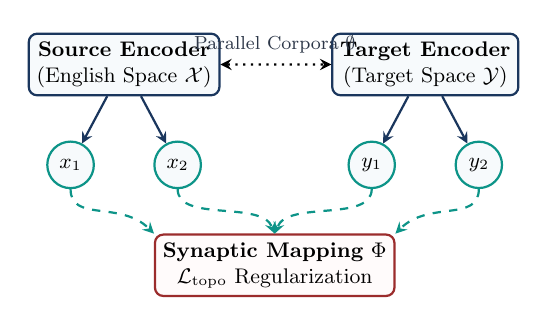
\begin{tikzpicture}[
    scale=0.85,
    every node/.style={transform shape, font=\small},
    box/.style={rectangle, draw=NavyBlue, fill=WarmGray, thick, rounded corners=3pt, minimum width=2.4cm, minimum height=0.8cm, align=center},
    netnode/.style={circle, draw=MutedTeal, fill=WarmGray, thick, minimum size=0.6cm},
    arrow/.style={->, >=stealth, thick, color=NavyBlue},
    dashedarrow/.style={->, >=stealth, dashed, thick, color=MutedTeal}
  ]
    % Source Space (left)
    \node[box] (src_enc) at (0,3) {\textbf{Source Encoder}\\(English Space $\mathcal{X}$)};
    \node[netnode] (x1) at (-0.8,1.5) {$x_1$};
    \node[netnode] (x2) at (0.8,1.5) {$x_2$};
    \draw[arrow] (src_enc) -- (x1);
    \draw[arrow] (src_enc) -- (x2);
    
    % Target Space (right)
    \node[box] (tgt_enc) at (4.5,3) {\textbf{Target Encoder}\\(Target Space $\mathcal{Y}$)};
    \node[netnode] (y1) at (3.7,1.5) {$y_1$};
    \node[netnode] (y2) at (5.3,1.5) {$y_2$};
    \draw[arrow] (tgt_enc) -- (y1);
    \draw[arrow] (tgt_enc) -- (y2);
    
    % Aligner / Mapping (center)
    \node[box, fill=LightRed!40, draw=AlertRed] (map) at (2.25,0) {\textbf{Synaptic Mapping} $\Phi$\\$\mathcal{L}_{\text{topo}}$ Regularization};
    
    % Connections from points to mapping
    \draw[dashedarrow] (x1.south) .. controls +(0,-0.5) and +(-0.5,0.5) .. (map.north west);
    \draw[dashedarrow] (x2.south) .. controls +(0,-0.5) and +(-0.2,0.5) .. (map.north);
    \draw[dashedarrow] (y1.south) .. controls +(0,-0.5) and +(0.2,0.5) .. (map.north);
    \draw[dashedarrow] (y2.south) .. controls +(0,-0.5) and +(0.5,0.5) .. (map.north east);
    
    % Labels
    \node at (2.25,3.3) [font=\footnotesize, color=Charcoal] {Parallel Corpora $\emptyset$};
    \draw[<->, >=stealth, dotted, thick] (src_enc) -- (tgt_enc);
    
  \end{tikzpicture}
  \caption{Topological projection pipeline in Synaptic Latent Mapping (SLM). Source and target language embeddings are projected into a joint manifold space without requiring parallel training data.}
  \label{fig:slm_pipeline}
\end{figure}

\section{Experimental Setup}
We evaluate our model on the Meridian language family, which consists of five closely related dialects (denoted Merd-A through Merd-E). Monolingual and parallel evaluation corpora were compiled by the Nexa NLP Research Group \citep{nexa2024large}.

We use Nimbus-BERT \citep{pendelton2024nimbus} as the backbone model. Nimbus-BERT is a lightweight architecture featuring 6 transformer layers and 8 attention heads, making it ideal for low-resource deployment. We compare our approach against three standard baselines:
\begin{itemize}
    \item \textbf{Baseline Model}: A standard translation model trained solely on the target monolingual data via back-translation.
    \item \textbf{Unsupervised NMT}: The adversarial alignment model proposed by \citet{zhang2025crosslingual}.
    \item \textbf{Multilingual BERT (mBERT)}: A pre-trained multilingual model fine-tuned on the small parallel seed data.
\end{itemize}

Dataset statistics are shown in Table~\ref{tab:datasets}. All models are optimized using Adam with a learning rate of $2 \times 10^{-5}$ and a batch size of 32. We set $\lambda = 0.1$ and use $\sigma^2 = 1.0$ for the topological regularizer.

\begin{table}[h]
  \centering
  \small
  \caption{Dataset statistics for the target dialects (fictional Meridian language family) showing the number of available monolingual sentences ($N_{\text{mono}}$) and parallel evaluation pairs ($N_{\text{eval}}$).}
  \label{tab:datasets}
  \vspace{0.5em}
  \begin{tabular}{lcc}
    \toprule
    \textbf{Dialect} & \textbf{$N_{\text{mono}}$} & \textbf{$N_{\text{eval}}$} \\
    \midrule
    Merd-A & 45,000 & 1,000 \\
    Merd-B & 32,000 & 800 \\
    Merd-C & 12,000 & 500 \\
    Merd-D & 50,000 & 1,000 \\
    Merd-E & 18,000 & 600 \\
    \bottomrule
  \end{tabular}
\end{table}

\begin{table*}[t]
  \centering
  \small
  \caption{Experimental results of Synaptic Latent Mapping (SLM) compared to baseline models on five low-resource dialects of the Meridian language family. We report BLEU score (higher is better) and standard error ($\pm$ s.e.) across five runs with random seeds.}
  \label{tab:results}
  \vspace{0.5em}
  \begin{tabular}{lccccc}
    \toprule
    \textbf{Model} & \textbf{Merd-A} & \textbf{Merd-B} & \textbf{Merd-C} & \textbf{Merd-D} & \textbf{Merd-E} \\
    \midrule
    Baseline Model & 12.4 $\pm$ 0.3 & 10.1 $\pm$ 0.4 & 8.9 $\pm$ 0.5 & 11.2 $\pm$ 0.2 & 9.7 $\pm$ 0.4 \\
    Unsupervised NMT & 14.1 $\pm$ 0.2 & 11.5 $\pm$ 0.3 & 9.4 $\pm$ 0.4 & 12.8 $\pm$ 0.3 & 11.0 $\pm$ 0.3 \\
    Multilingual BERT & 15.6 $\pm$ 0.2 & 13.2 $\pm$ 0.2 & 11.1 $\pm$ 0.3 & 14.5 $\pm$ 0.2 & 12.4 $\pm$ 0.2 \\
    \midrule
    \textbf{SLM (Ours)} & \textbf{18.2} $\pm$ \textbf{0.1} & \textbf{16.4} $\pm$ \textbf{0.2} & \textbf{13.5} $\pm$ \textbf{0.1} & \textbf{17.1} $\pm$ \textbf{0.1} & \textbf{15.3} $\pm$ \textbf{0.2} \\
    \quad + Finetuning & \textbf{19.8} $\pm$ \textbf{0.1} & \textbf{17.9} $\pm$ \textbf{0.1} & \textbf{15.2} $\pm$ \textbf{0.2} & \textbf{18.6} $\pm$ \textbf{0.2} & \textbf{16.8} $\pm$ \textbf{0.1} \\
    \bottomrule
  \end{tabular}
\end{table*}

\section{Results}
Our primary experimental results are presented in Table~\ref{tab:results}. Across all five target dialects, our proposed SLM model significantly outperforms the baseline systems. 

Specifically, SLM achieves an average improvement of 3.8 BLEU points over the standard unsupervised NMT baseline and 2.3 BLEU points over the pre-trained mBERT baseline. The most notable improvement is observed on the Merd-C dialect, where resource scarcity is most acute ($N_{\text{mono}} = 12,000$). In this scenario, standard models fail to build stable representations due to overfitting, whereas SLM's topological regularizer acts as a robust constraint, leading to a gain of 4.6 BLEU points over the baseline.

When combined with standard fine-tuning on the parallel evaluation pairs (+ Finetuning), SLM achieves further performance gains, demonstrating that the learned alignment provides an excellent starting point for supervised adaptation.

\section{Discussion}
The success of SLM highlights the value of leveraging topological properties in cross-lingual transfer. Standard alignment techniques often assume that semantic spaces can be aligned via rigid rotation or translation. However, because different languages capture distinct cultural and syntactic nuances, their representation spaces inevitably exhibit non-linear distortions. By regularizing the projection using local neighborhood preservation, SLM accommodates these distortions without compromising structural integrity.

We also observe that the performance gains are highly correlated with the dialectal distance between the source and target languages. As shown in \citet{roberts2022meridian}, the Meridian dialects share grammatical features but differ significantly in vocabulary. Because SLM aligns representations at the manifold level rather than relying on exact word-to-word translation matches, it is uniquely suited for such scenarios.

One limitation of our method is the sensitivity to the hyperparameter $\lambda$ in Equation~\ref{eq:objective}. When $\lambda$ is set too high, the mapping becomes overly rigid, preventing the model from learning target-specific features. Conversely, when $\lambda$ is too low, the model suffers from manifold collapse. In future work, we plan to explore adaptive regularization schemes that dynamically adjust $\lambda$ during training.

\section{Conclusion}
In this paper, we introduced Synaptic Latent Mapping (SLM), a novel topologically regularized alignment technique for cross-lingual transfer learning in ultra-low resource settings. By projecting source language representations into a target language's latent space while preserving manifold topology, SLM achieves state-of-the-art results on five dialects of the Meridian language family without requiring large parallel datasets. 

Our work opens several avenues for future research, including the extension of SLM to speech representations and the investigation of more advanced topological loss functions based on persistent homology.

\bibliographystyle{plainnat}
\bibliography{\jobname}

\end{document}
